\documentclass{../lab_class}

\usepackage{fancyhdr}
\pagestyle{fancy}
\rhead{П.\,Ю. Смирнов, 687 гр.}
\lhead{Лабораторная работа № 3.3.5, МФТИ, осень 2017}

\begin{document}

{\Large 3.3.5 -- Эффект Холла в металлах.}

\paragraph{Цель работы.}
Измерение подвижности и концентрации носителей зарядов в металлах.

В работе используются: электромагнит с источником питания, источник постоянного тока, микровольтметр, амперметры, милливеберметр, образцы из серебра и цинка.

\paragraph{Теоретическая часть.}
Ещё по полуклассической теории Бора мы знаем, что энергия электронов в атомах квантуется. Несомненно, твердое тело как макроскопическое объединение отдельных атомов имеет гораздо более сложную структуру, чем отдельный атом; тем не менее, с большой степенью точности поведение электронов в твердом теле можно описать, используя \emph{зонную модель}. В ней мы предполагаем, что каждый электрон суть <<общий>> для всех атомов данного твердого тела объект, имеющий дискретное распределение энергии (конечно, отличное от такового для отдельного атома). Вместо уровней теперь речь идёт о т.~н. зонах. Верхняя из заполненных зон -- \emph{валентная зона}; верхняя незаполненная зона -- \emph{зона подвижности}. Если все зоны заполнены, твердое тело суть диэлектрик; в противном случае оно проводник или полупроводник, в зависимости от того, как сильно заполнена зона подвижности. Во внешнем электрическом поле электроны в подвижной зоне, как ясно из данного названия, приходят в движение. Для удобства его описания обычно вводят \emph{дырки} -- квазичастицы, имеющие смысл отсутствия электрона в кристаллической решетке. Поэтому мы используем далее термин \emph{носитель заряда}, хотя де-факто есть только один вид носителя -- электрон.

\begin{wrapfigure}[12]{r}{5.5cm}
	\centering
	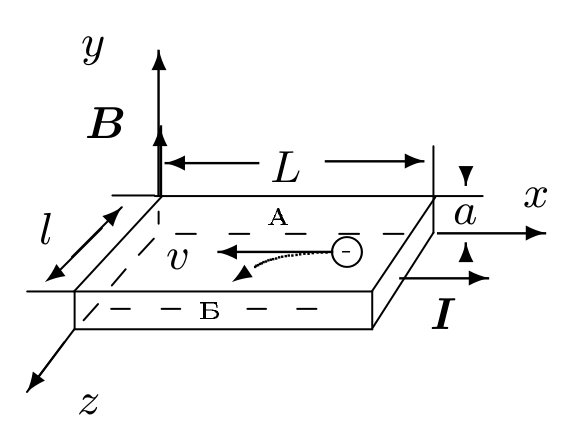
\includegraphics[width=5.5cm]{on_hall.png}
	\caption{К рассмотрению эффекта Холла}
	\label{fig:hall}
\end{wrapfigure}

Как же движутся носители заряда? Во многом похоже на механизм переноса субстанции в явлениях трения, теплопроводности и диффузии. Носитель ускоряется под действием электрического поля, проходит некоторую <<длину свободного пробега>>, врезается в какой-нибудь узел решетки, теряет скорость, и всё по новой. При этом при данных постоянных условиях (однородность вещества, постоянная температура, напряженность поля и т.~п.) можно считать, что
\begin{equation*}
	\avg{\vb{v}} = -b \vb{E},
\end{equation*}
где $b$ -- \emph{подвижность}. Пусть $n$ -- средняя концентрация носителей заряда, $e$ -- их заряд. Для плотности тока получаем тогда
\begin{equation*}
	j = n e \avg{v} = e n b E = \sigma E,
\end{equation*}
где $\sigma = e n b$ -- \emph{проводимость}. 

Мы видим, что в нашей модели\footnote{Внимательный читатель может заметить, что при <<выводе>> закона Ома и эффекта Холла мы никак не пользуемся положениями зонной теории. Бесспорно, эта теория неплохо описывает физику твердого тела качественно, однако мы не в состоянии привести ни одного количественного закона. Фактически, мы пользуемся здесь классической теорией Друде, созданной по образу и подобию кинетической теории газов (электронный газ и т.~п.).} выполняется закон Ома. С этим уже можно работать, ибо измерить проводимость -- дело простое. Заряд носителей мы знаем -- это заряд электрона, известный нам по опыту Милликена\footnote{Хотя я его не воспроизводил.}.

Ещё немного информации можно получить, если поместить образец с током в постоянное магнитное поле так, как это показано на рисунке \ref{fig:hall}. Ведь тогда на носители заряда в металле будет действовать сила Лоренца $F = e \abs{\avg{v_x}} B$, смещающая их вдоль оси $z$. Это приводит к накоплению избыточного заряда одного знака на боковых гранях А и Б пластины. Избыточный заряд, в свою очередь, создает электрическое поле, препятствующее дальнейшему накоплению заряда -- и так до тех пор, пока обе силы не уравновесят друг друга. Произойдет это, понятно, когда $E_z = \abs{\avg{v_x}} B$; в таком случае между боковыми гранями создаётся некоторое \emph{холловское напряжение} $U = -E_z l$.

\pagebreak

Замечая, что сила тока есть
\begin{equation*}
	I = n e \abs{\avg{v_x}} l a,
\end{equation*}
получаем выражение для ЭДС Холла в виде
\begin{equation}\label{eq:hall_voltage}
	U = - \frac{IB}{nea} = -R_H \frac{IB}{a},
\end{equation}
где $R_H = 1/ne$ -- \emph{постоянная Холла}. Что же мы видим? Измерение проводимости среды позволяет определить произведение $enb$, а исследование эффекта Холла -- $en$. Раз мы знаем заряд электрона, то, следовательно, можем получить из данных опытов информацию о концентрации носителей (электронов или дырок) и их подвижности, следовательно, косвенно о структуре твердого тела. Этим и займемся.

\paragraph{Экспериментальная установка.}
Суть проста -- вносим металлическую пластину в зазор электромагнита и измеряем микровольметром ЭДС Холла. Сила тока через пластину регулируется реостатом.

\begin{figure}[H]
	\centering
	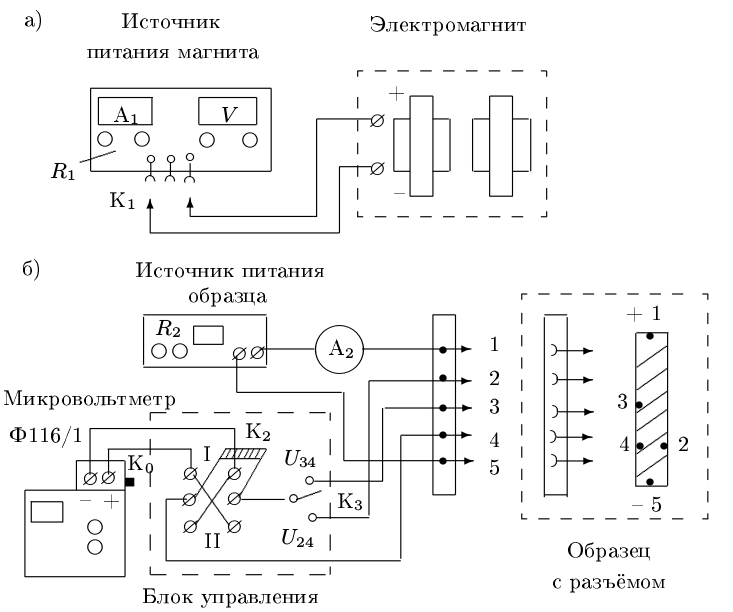
\includegraphics[width = 0.6 \textwidth]{scheme.png}
	\caption{Схема экспериментальной установки}
	\label{fig:schemet}
\end{figure}


\end{document}